\documentclass[11pt,a4paper]{article}

\usepackage{fontspec}
\setmainfont{Times New Roman}
\usepackage[russian]{babel}

\usepackage[left=20mm,right=15mm,top=15mm,bottom=15mm]{geometry}
\usepackage{amsmath,amssymb,amsfonts}
\usepackage{graphicx}
\usepackage{booktabs}
\usepackage{caption}
\usepackage{subcaption}
\usepackage{hyperref}
\usepackage{microtype}
\usepackage{float}

\hypersetup{
    colorlinks=true,
    linkcolor=black,
    urlcolor=blue,
    citecolor=black
}

\setlength{\parindent}{1.25cm}
\setlength{\parskip}{0.15em}
\linespread{1.1}
\setlength{\abovedisplayskip}{3pt}
\setlength{\belowdisplayskip}{3pt}

\begin{document}

% -------------------------------------------------------------
% ТИТУЛЬНЫЙ ЛИСТ
% -------------------------------------------------------------
\begin{titlepage}
    \centering
    {\bfseries\large Белорусский государственный университет\par}
    {\bfseries\large Факультет прикладной математики и информатики\par}
    
    \vspace{6cm}
    {\Huge\bfseries ОТЧЁТ\par}
    \vspace{0.5cm}
    {\large по лабораторной работе №3 по компьютерной графике\par}
    \vspace{0.5cm}
    {\Large\bfseries Базовые растровые алгоритмы: пошаговый алгоритм, ЦДА, алгоритмы Брезенхема\par}
    
    \vspace{6cm}
    \begin{flushright}
        \large
        \textbf{Выполнил:}\\
        студент 4 группы 3 курса\\
        Дикан Д.~А.\\[1em]
        \textbf{Преподаватель:}\\
        старший преподаватель\\
        Соловей Сергей Сергеевич
    \end{flushright}
    
    \vfill
    {\large Минск, 2026\par}
\end{titlepage}

\newpage

% -------------------------------------------------------------
% СТРАНИЦА 2: ЦЕЛЬ И ТЕОРИЯ
% -------------------------------------------------------------
\section*{1. Цель работы}
Изучить базовые алгоритмы растеризации отрезка (пошаговый алгоритм, цифровой дифференциальный анализатор, алгоритм Брезенхема) и окружности (алгоритм Брезенхема), провести сравнительный анализ их точности и времени работы, а также разработать веб-приложение для наглядной визуализации дискретной координатной сетки с протоколом вычислений.

\section*{2. Теоретические сведения}
\begin{enumerate}
    \item \textbf{Растровая сетка.} Пикселю с целочисленными координатами $(x, y)$ соответствует ячейка непрерывной плоскости $[x, x + 1) \times [y, y + 1)$ с центром в точке $(x + 0.5, \, y + 0.5)$. Задача растеризации заключается в выборе тех пикселей, центры которых минимизируют расстояние до идеальной математической линии.

    \item \textbf{Пошаговый алгоритм.} Основан на прямом вычислении уравнения прямой:
    \begin{equation}
        y = k \cdot x + b, \quad \text{где } k = \frac{\Delta y}{\Delta x}, \quad b = y_1 - k \cdot x_1.
    \end{equation}
    При $|k| \le 1$ ведущей является ось $Ox$ (шаг $s = \operatorname{sign}(\Delta x)$):
    \begin{equation}
        x_{i+1} = x_i + s, \quad y_{i+1} = y_i + k \cdot s, \quad \text{пиксель: } \bigl(x_{i+1}, \, \operatorname{round}(y_{i+1})\bigr).
    \end{equation}
    При $|k| > 1$ ведущей становится ось $Oy$ (шаг по $y$, вычисление $x = (y - b) / k$).

    \item \textbf{Алгоритм ЦДА (Цифровой дифференциальный анализатор).} Длина проекции отрезка задает необходимое число шагов:
    \begin{equation}
        L = \max\bigl(|\Delta x|, \, |\Delta y|\bigr).
    \end{equation}
    Инкрементальные приращения координат на один шаг составляют:
    \begin{equation}
        \delta x = \frac{\Delta x}{L}, \quad \delta y = \frac{\Delta y}{L}.
    \end{equation}
    Рекуррентное соотношение для координат и итогового пикселя:
    \begin{equation}
        x_{i+1} = x_i + \delta x, \quad y_{i+1} = y_i + \delta y, \quad \text{пиксель: } \bigl(\operatorname{round}(x_{i+1}), \, \operatorname{round}(y_{i+1})\bigr).
    \end{equation}

    \item \textbf{Алгоритм Брезенхема для отрезка.} Для базового сектора $0 \le \Delta y \le \Delta x$ начальное значение разностного целочисленного параметра ошибки равно:
    \begin{equation}
        e_0 = 2\Delta y - \Delta x.
    \end{equation}
    Итерационный пересчет ошибки и выбор следующего пикселя:
    \begin{equation}
        e_{i+1} = \begin{cases}
            e_i + 2\Delta y, & \text{если } e_i < 0 \quad (\text{шаг } x \leftarrow x + 1), \\
            e_i + 2(\Delta y - \Delta x), & \text{если } e_i \ge 0 \quad (\text{шаг } x \leftarrow x + 1, \, y \leftarrow y + 1).
        \end{cases}
    \end{equation}
    Все операции выполняются строго в целых числах без операций деления и вещественного типа данных.

    \item \textbf{Алгоритм Брезенхема для окружности.} Каноническое уравнение окружности $x^2 + y^2 = R^2$ разбивается координатными осями и диагоналями $x = \pm y$ на 8 октантов (по 2 в каждой из 4 четвертей). Для сектора от $0^\circ$ до $45^\circ$ ($0 \le x \le y$ при начальной точке $(0, R)$) начальное значение решающей функции:
    \begin{equation}
        d_0 = 3 - 2R.
    \end{equation}
    Итерационный пересчет:
    \begin{equation}
        d_{i+1} = \begin{cases}
            d_i + 4x_i + 6, & \text{если } d_i < 0 \quad (\text{шаг вправо: } x \leftarrow x + 1), \\
            d_i + 4(x_i - y_i) + 10, & \text{если } d_i \ge 0 \quad (\text{шаг по диагонали: } x \leftarrow x + 1, \, y \leftarrow y - 1).
        \end{cases}
    \end{equation}
    Остальные 7 октантов формируются синхронным отражением: $(\pm x, \, \pm y)$ и $(\pm y, \, \pm x)$.
\end{enumerate}

\newpage

% -------------------------------------------------------------
% СТРАНИЦА 3: АРХИТЕКТУРА И РЕЗУЛЬТАТЫ
% -------------------------------------------------------------
\section*{3. Архитектура и реализация приложения}
\begin{itemize}
    \item \textbf{Серверная часть (Python 3, Flask):} модуль \texttt{processing.py} содержит функции генерации растровых точек и протокола шагов, модуль \texttt{main.py} реализует веб-контроллер с JSON API \texttt{/api/rasterize}.
    \item \textbf{Клиентская часть (HTML5, Tailwind CSS, Canvas API):} интерактивный холст с координатной сеткой, пикселями, непрерывной линией, переключением алгоритмов и трассировкой.
\end{itemize}

\section*{4. Результаты работы приложения}
На рисунке 1 представлен общий вид интерфейса разработанного приложения. На рисунках 2 и 3 показаны увеличенные фрагменты дискретной координатной сетки при растеризации отрезка и окружности алгоритмами Брезенхема:

\begin{figure}[H]
    \centering
    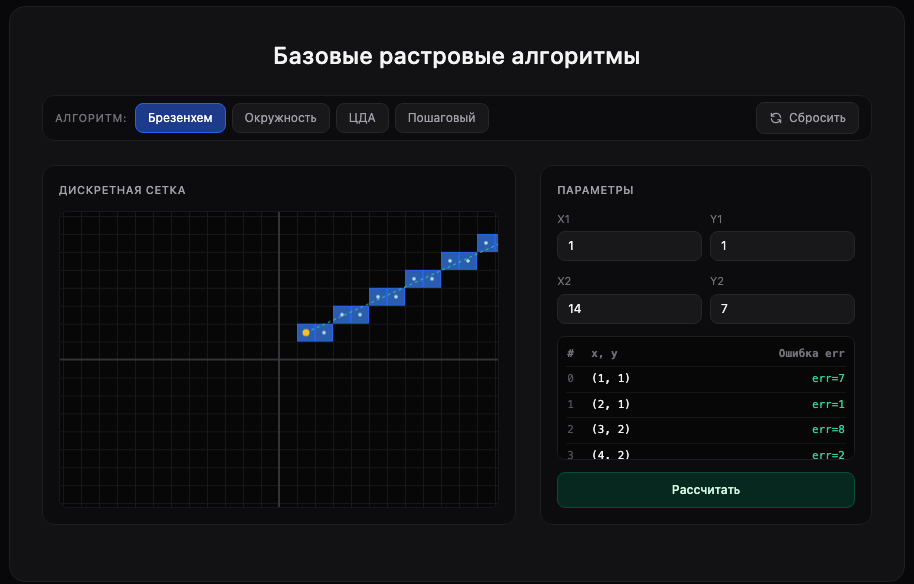
\includegraphics[width=0.55\textwidth]{../images/00_ui_overview.png}
    \caption{Общий вид интерфейса разработанного веб-приложения}
\end{figure}

\begin{figure}[H]
    \centering
    \begin{subfigure}[b]{0.42\textwidth}
        \centering
        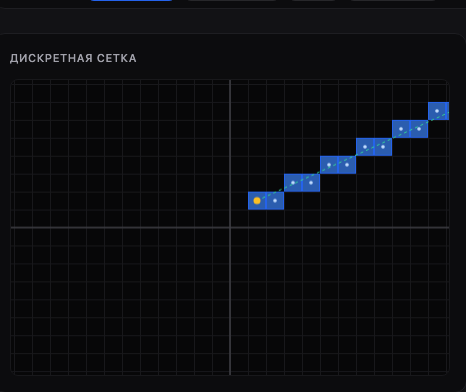
\includegraphics[width=\textwidth]{../images/01_canvas_line.png}
        \caption{Растеризация отрезка $(1, 1) \to (14, 7)$}
    \end{subfigure}
    \hfill
    \begin{subfigure}[b]{0.42\textwidth}
        \centering
        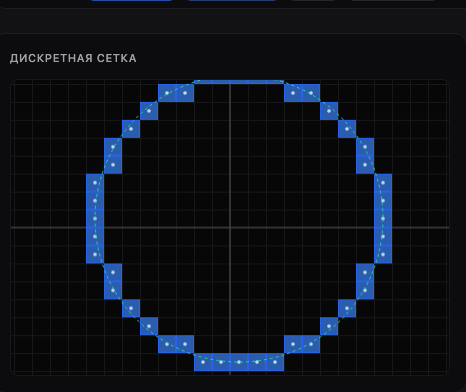
\includegraphics[width=\textwidth]{../images/02_canvas_circle.png}
        \caption{Растеризация окружности $(0, 0), \, R = 8$}
    \end{subfigure}
    \caption{Фрагменты дискретной сетки при растеризации примитивов}
\end{figure}

\newpage

% -------------------------------------------------------------
% СТРАНИЦА 4: ВРЕМЕННЫЕ ХАРАКТЕРИСТИКИ И ВЫВОДЫ
% -------------------------------------------------------------
\section*{Временные характеристики и сравнение методов}
В соответствии с заданием проведено измерение времени работы реализованных функций на наборе из 1000 произвольных отрезков с координатами в диапазоне $[-100, 100]$:

\begin{table}[H]
\centering
\begin{tabular}{@{}llp{8.5cm}@{}}
\toprule
\textbf{Алгоритм} & \textbf{Время (1000 линий)} & \textbf{Особенности реализации в коде} \\
\midrule
\textbf{Алгоритм Брезенхема} & \textbf{10.9 мс} & Самый быстрый: только сложение, вычитание целых чисел и сдвиги. \\
\textbf{Пошаговый алгоритм}  & \textbf{22.7 мс} & Арифметика с плавающей точкой (float) и вызов функции \texttt{round()} на каждом шаге. \\
\textbf{Алгоритм ЦДА}        & \textbf{27.8 мс} & Сложение с вещественными приращениями $\delta x, \delta y$ и вызовы округления \texttt{round()}. \\
\bottomrule
\end{tabular}
\end{table}

\textbf{Точность растра:} все три алгоритма аппроксимируют отрезок с максимальным отклонением центра пикселя от непрерывной прямой не более $0.5000$ пикселя (среднее отклонение составляет $0.2441$ пикселя, а среднее евклидово расстояние~--- $0.2205$ пикселя). Все методы дают свыше $99.4\%$ идентичных пикселей. Редкие расхождения (менее $0.6\%$ случаев) возникают только тогда, когда линия проходит точно посередине между двумя пикселями (при значении $0.5$), где Брезенхем выбирает верхний пиксель, а функция \texttt{round()} в Python округляет к ближайшему четному числу.

\section*{5. Выводы}
\begin{enumerate}
    \item \textbf{Качество растеризации.} Все три алгоритма дают визуально идентичный результат: расхождения в выборе пикселя встречаются только в пограничных случаях, когда прямая проходит ровно между двумя клетками. Это подтверждает, что разница между методами~--- вычислительная, а не геометрическая.
    \item \textbf{Целочисленная арифметика быстрее.} На 1000 отрезках Брезенхем оказался в $2$--$2.5$ раза быстрее ЦДА и пошагового метода. Преимущество достигается исключительно за счет замены деления и умножения сложением и побитовым сдвигом, без потери точности.
    \item \textbf{Симметрия сокращает вычисления.} Благодаря 8-кратной симметрии окружности достаточно вычислить координаты лишь одной восьмой контура. Остальные семь частей получаются отражением, что снижает число итераций с $\sim 2\pi R$ до $\sim R / \sqrt{2}$.
    \item \textbf{Область применения ЦДА.} Несмотря на проигрыш в скорости, ЦДА удобен там, где вдоль ребра нужно интерполировать дополнительные параметры~--- цвет или текстурные координаты~--- поскольку дробный шаг уже есть в переменных алгоритма.
\end{enumerate}

\end{document}
